\documentclass[10pt]{beamer}

\usepackage[brazilian]{babel}
\usepackage[utf8]{inputenc}
\usepackage{graphicx}
\usepackage{mathtools}
\usepackage{amsthm}
\usepackage{thmtools,thm-restate}
\usepackage{amsfonts}
\usepackage{hyperref}
\usepackage[singlelinecheck=false]{caption}
\usepackage[backend=biber,url=true,doi=true,eprint=false,style=alphabetic]{biblatex}
\usepackage[justification=centering]{caption}
\usepackage{indentfirst}
\usepackage{enumitem}
\usepackage{algorithm}
\usepackage{algpseudocode}
\usepackage{listings}

%remove line breaks
\setbeamertemplate{bibliography entry title}{}
\setbeamertemplate{bibliography entry location}{}
\setbeamertemplate{bibliography entry note}{}

\uselanguage{Brazilian}
\languagepath{Brazilian}
\usetheme{Berlin}

\addbibresource{references.bib}

\newcommand\nmfootnote[1]{%
  \begingroup
  \renewcommand\thefootnote{}\footnote{#1}%
  \addtocounter{footnote}{-1}%
  \endgroup
}

\makeatletter
\def\subsection{\@startsection{subsection}{3}%
  \z@{.5\linespacing\@plus.7\linespacing}{.1\linespacing}%
  {\normalfont\itshape}}
\makeatother

\DeclareMathOperator*{\argmin}{arg\,min}
\DeclareMathOperator*{\argmax}{arg\,max}

\newcommand\defeq{\mathrel{\overset{\makebox[0pt]{\mbox{\normalfont\tiny\sffamily def}}}{=}}}

\floatname{algorithm}{Algoritmo}
\algrenewcommand\algorithmicrequire{\textbf{Input}}
\algrenewcommand\algorithmicensure{\textbf{Output}}

\captionsetup[table]{labelsep=space}

\theoremstyle{plain}

\newtheorem{proposition}{Proposição}
\newtheorem{exercise}{Exercício}

\newcommand{\set}[1]{\mathbf{#1}}
\newcommand{\pr}{\mathbb{P}}
\renewcommand{\implies}{\Rightarrow}

\newcommand{\bigo}{\mathcal{O}}
\newcommand{\p}{\pause}

\setlength{\parskip}{1em}

\lstset{frameround=fttt,
  language=[5.3]Lua,
  numbers=left,
  breaklines=true,
  keywordstyle=\bfseries,
  basicstyle=\ttfamily,
}

\newcommand\Fontsmall{\fontsize{12}{7.2}\selectfont}

\newcommand{\code}[1]{\lstinline[mathescape=true]{#1}}
\newcommand{\mcode}[1]{\lstinline[mathescape]!#1!}

\title{Estudo sobre Sum-Product Networks e Aprendizagem Profunda}
\author{Renato Lui Geh}
\institute[IME-USP] {%
  Instituto de Matemática e Estatística\\
  Universidade de São Paulo
}
\titlegraphic{\hspace*{7.5cm}~
\includegraphics[scale=0.25]{imgs/logo.png}}

\begin{document}

\frame{\titlepage}

\begin{frame}
  \frametitle{Índice}
  \tableofcontents
\end{frame}

%--------------------------------------------------------------------------------------------------

\section{Definição}

\begin{frame}
  \frametitle{Relembrando$\ldots$}
  \begin{definition}\label{pd-def}
    Uma SPN $S$ é um DAG com três tipos de nós: soma, produto e indicadores. Todo nó indicador é uma
    folha. Todo nó soma tem pais produto, e todo nó produto tem pais soma. Toda aresta com destino a
    um nó soma tem uma aresta com um peso associado. O valor de um nó soma $i$ é $\sum_{j\in Ch(i)}
    w_{ij}v_j$ e o valor de um nó produto $i$ é $\prod_{j\in Ch(i)}v_j$, onde $Ch(i)$ é o conjunto
    de filhos de $i$, $v_i$ é o valor do nó $i$ e $w_{ij}$ é o peso associado a aresta $i\to j$. Uma
    SPN representa um \emph{network polynomial} de uma distribuição de probabilidade, e os
    indicadores da função são as folhas da SPN\@. O valor de uma SPN é o valor do nó raíz.
  \end{definition}\nmfootnote{\cite{poon-domingos}}
\end{frame}

\begin{frame}
  \frametitle{Relembrando$\ldots$}
  \begin{figure}[h]
    \centering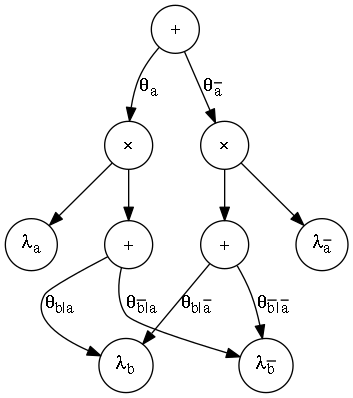
\includegraphics[scale=0.3]{imgs/simple_spn.png}
  \end{figure}
\end{frame}

\begin{frame}
  \frametitle{Sub-SPNs}
  \begin{proposition}
    Seja um nó arbitrário $i$ de uma SPN $S$, então $S_i$ é uma sub-SPN que tem nó raíz em $i$.
  \end{proposition}
\end{frame}

\begin{frame}
  \frametitle{Prova sub-SPNs}
  \begin{proof}
    Considere o caso base em que $i$ é um nó indicador. Um nó indicador é uma distribuição de
    probabilidade monovariável. Portanto $i$ é uma distribuição de probabilidade e pode ser
    representada por uma SPN, que no caso possue apenas um nó.

    Se $i$ é um nó soma, então o valor de $i$ é $v_i=\sum_{j\in Ch(i)} w_{ij}v_j$. A soma de várias
    distribuições de probabilidade é uma distribuição de probabilidade. Portanto um nó soma é
    representável por uma SPN\@.

    Caso $i$ seja um nó produto, então o valor de $i$ é $v_i=\sum_{j\in Ch(i)} v_j$. A multiplicação
    de distribuições de probabilidade é bem definida e é uma distribuição de probabilidade. Um nó
    produto é uma SPN\@.
  \end{proof}
\end{frame}

%--------------------------------------------------------------------------------------------------

\section{Propriedades}

\begin{frame}
  \frametitle{Completude}
  \begin{definition}[Completude]
    Uma SPN $S$ é completa se e somente se, para todo nó soma $i$, o escopo de $i$ é igual par-a-par
    $Sc(S_i)=Sc(S_j)$ ao escopo de cada filho $j\in Ch(i)$.
  \end{definition}
\end{frame}

\begin{frame}
  \frametitle{Consistência}
  \begin{definition}[Consistência]
    Uma SPN $S$ é consistente se e somente se, para todo nó produto $i$, nenhum filho de $i$ tem
    valor diferente dos outros filhos.
  \end{definition}
\end{frame}

\begin{frame}
  \frametitle{Validade}
  \begin{definition}[Validade]
    Uma SPN $S$ é válida se $S$ é consistente e completa.
  \end{definition}
\end{frame}

\begin{frame}
  \frametitle{Decomponibilidade}
  \begin{definition}[Decomponibilidade]
    Uma SPN $S$ é decomponível se e somente se, para cada par $c_1, c_2 \in Ch(i)$ para qualquer $i$
    nó produto em $S$, $Sc(c_1)\cap Sc(c_2)=\emptyset$.
  \end{definition}
\end{frame}

%--------------------------------------------------------------------------------------------------

\section{Uma definição alternativa}

\begin{frame}
  \frametitle{Uma definição alternativa}
  \begin{definition}\label{gd-def}
    Uma SPN tem uma definição recursiva. Definimos que uma SPN $S_i$ pode ser apenas:
    \begin{enumerate}[label=(\roman*)]
      \item\label{gd-ref-1} Uma distribuição monovariável $p(\set{X})$ ou;
      \item\label{gd-ref-2} Um nó soma tal que $S_i=\sum_{j\in Ch(i)} w_{ij}v_j$ onde para cada filho
        $j,k\in Ch(i)$, $Sc(S_j)=Sc(S_k)$ ou;
      \item\label{gd-ref-3} Um nó produto tal que $S_i=\prod_{j\in Ch(i)} v_j$ onde para cada filho
        $j,k\in Ch(i)$, $Sc(S_j)\cap Sc(S_k)=\emptyset$.
    \end{enumerate}
  \end{definition}\nmfootnote{\cite{gens-domingos}}
\end{frame}

\begin{frame}
  \frametitle{Uma definição alternativa}
  \begin{figure}[h]
    \centering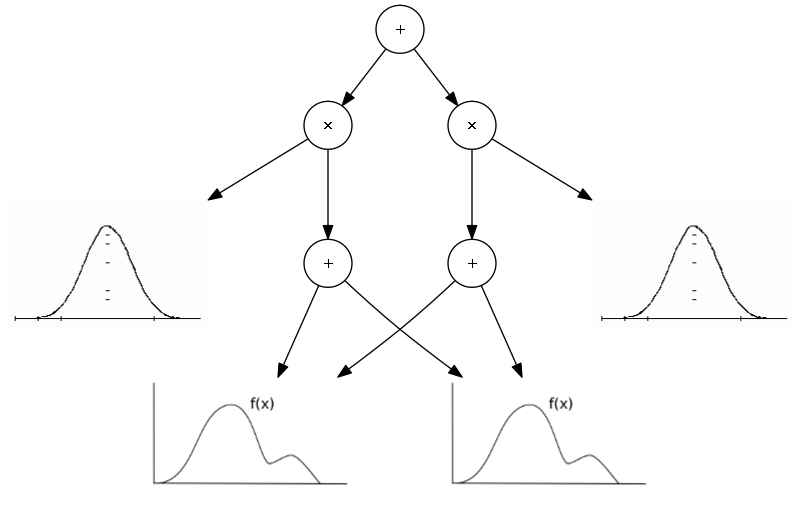
\includegraphics[scale=0.3]{graphs/alt_spn.png}
  \end{figure}
\end{frame}

%--------------------------------------------------------------------------------------------------

\section{Classificação por Naive Bayes}

\begin{frame}
  \frametitle{Classificação por Naive Bayes}
  \begin{flalign*}
    C &: \text{~variável classe}&\\
    \set{A}=\{A_1,\ldots,A_n\} &: \text{~variáveis atributos}&
  \end{flalign*}
  $A_i\perp A_j \equiv A_i\perp_d A_j$, para $1 \leq i,j\leq n$ e $i\neq j$
  \begin{figure}[h]
    \centering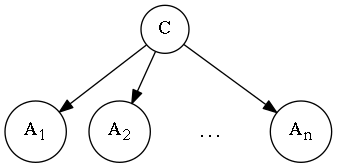
\includegraphics[scale=0.3]{graphs/naivebayes.png}
  \end{figure}
\end{frame}

\begin{frame}
  \frametitle{Classificação por Naive Bayes}
  Pelo Teorema da Fatorização:
  \begin{equation*}
    \Pr(C,A_1,\ldots,A_n)=\Pr(C)\prod_{i=1}^n \Pr(A_i|C)
  \end{equation*}
  Classificação resume-se a encontrar um máximo $c$:
  \begin{equation*}
    \argmax_c\left(\Pr(C=c|A_1=a_1,\ldots,A_k=a_k)=\frac{\Pr(C=c,A_1,\ldots,A_k=a_k)}{\Pr(A_1=a_1,
    \ldots,A_k=a_k)}\right)
  \end{equation*}
\end{frame}

\begin{frame}
  \frametitle{Aprendizado de Naive Bayes por MLE}
  MLE (Maximum Likelihood Estimation) $\equiv$ Máxima verossimilhança

  Aprender uma Naive Bayes:
  \begin{description}
    \item[Variável classe] $\Pr(C=c)=\frac{N[C=c]}{N}$
    \item[$i$-ésimo atributo] $\Pr(A_i=a_i|C=c)=\frac{N[A_i=a_i,C=c]}{N[C=c]}$
  \end{description}
\end{frame}

%--------------------------------------------------------------------------------------------------

\section{Aprendizado estrutural de SPNs}

\begin{frame}
  \frametitle{Aprendizado estrutural de SPNs}
  \begin{algorithm}[H]
    \caption{LearnSPN~\cite{gens-domingos}}\label{learn-alg}
    \begin{algorithmic}[1]
      \Require~Conjunto $\set{X}$ de variáveis, conjunto $\set{I}$ de instâncias
      \Ensure~Uma SPN resultante do aprendizado estrutural
      \If{$|\set{X}|=1$}
        \State~Retorna uma distribuição monovariável de $\set{X}$
      \EndIf
      \State~Tente dividir as variáveis $\set{X}$ em duas partições $\set{X}_1$ e $\set{X}_2$ onde
        $\set{X}_1$ é (aproximadamente) independente de $\set{X}_2$
      \If{dá para dividir}
        \State~\textbf{return} $\prod_{i=1}^2$ LearnSPN($\set{X}_i$, $\set{I}$)
      \Else
        \State~Divida as instâncias $\set{I}$ em partições $\set{I}_1$ e $\set{I}_2$ tal que
          $\set{I}_1$ e $\set{I}_2$ sejam o mais similares possíveis.
        \State~\textbf{return} $\sum_{i=1}^2 \frac{|\set{I}_i|}{|\set{I}|}$ LearnSPN($\set{X}$,
          $\set{I}_i$)
      \EndIf
    \end{algorithmic}
  \end{algorithm}
\end{frame}

%--------------------------------------------------------------------------------------------------

\section[Referências]{Referências e Bibliografia}
\begin{frame}[t,allowframebreaks]
  \frametitle{Referências e Bibliografia}
  \footnotesize
  \printbibliography[]
\end{frame}

\end{document}
